%%%%%%%%%%%%%%%%%%%%%%%%%%%%%%%%%%%%%%%%%%%%%%%%%%%%%%%%%%%%%%%%%%%%%%%%%%%%%%%%
% Thesis / Project Report
% LaTeX Template
% Version 2.0 (08/04/16)
%
% Author:
% Siddhant Shrivastava
% https://github.com/sidcode/bits-pilani-thesis-template-latex
%
% This template is heavily based on the work of Darshit Shah, Steven Gunn and Sunil Patel
% Darshit Shah
% https://github.com/darnir/BPHC-LaTeX-Report-Class
% Steven Gunn
% http://users.ecs.soton.ac.uk/srg/softwaretools/document/templates/
% and
% Sunil Patel
% http://www.sunilpatel.co.uk/thesis-template/
%
% License:
% CC BY-NC-SA 4.0 (http://creativecommons.org/licenses/by-nc-sa/4.0/)
%
% Note:
% Make sure to edit document variables in the Thesis.cls file
%
%%%%%%%%%%%%%%%%%%%%%%%%%%%%%%%%%%%%%%%%%%%%%%%%%%%%%%%%%%%%%%%%%%%%%%%%%%%%%%%%

%-------------------------------------------------------------------------------
%	PACKAGES AND OTHER DOCUMENT CONFIGURATIONS
%-------------------------------------------------------------------------------

\documentclass[11pt, a4paper, oneside]{Thesis} % Paper size, default font size
% and one-sided paper

\graphicspath{{Pictures/}} % Specifies the directory where pictures are stored

\usepackage[backend=bibtex]{biblatex}
\usepackage{textcomp}
\usepackage[T1]{fontenc}
\usepackage{lmodern}
\bibliography{Bibliography.bib}

\title{\ttitle} % Defines the thesis title - don't touch this

\begin{document}
	
	\frontmatter % Use roman numbering style (i, ii...) for the pre-content pages
	
	\setstretch{1.3} % Line spacing of 1.3
	
	% Define page headers using FancyHdr package and set up for one-sided printing
	\fancyhead{} % Clears all page headers and footers
	\rhead{\thepage} % Sets the right side header to show the page number
	\lhead{} % Clears the left side page header
	
	\pagestyle{fancy} % Finally, use the "fancy" page style to implement the
	%FancyHdr headers
	
	% Input all the variables used in the document. Please fill out the
	% variables.tex file with all your details.
	%-------------------------------------------------------------------------------
%	DOCUMENT VARIABLES
%
%	Fill in the lines below to set the various variables for the document
%-------------------------------------------------------------------------------

%-------------------------------------------------------------------------------
% Your thesis title - this is used in the title and abstract
% Command: \ttitle
\thesistitle{Designing A Reliable Real Time Feed Listener}
%-------------------------------------------------------------------------------
% The document type: Thesis / report, etc.
% Command: \doctype
\documenttype{Mid Semester Report}
%-------------------------------------------------------------------------------
% Your supervisor's name - this is used in the title page
% Command: \supname
\supervisor{Chetan \textsc{Dugar}}
%-------------------------------------------------------------------------------
% The supervisor's position - Used on Certificate
% Command: \suppos
\supervisorposition{Software Engineer III}
%-------------------------------------------------------------------------------
% Supervisor's institute
% Command: \supinst
\supervisorinstitute{Tower Research Capital LLC, Gurgaon}
%-------------------------------------------------------------------------------
% Your Co-Supervisor's name
% Command: \cosupname
\cosupervisor{Gaurab \textsc{Basu}}
%-------------------------------------------------------------------------------
% Co-Supervisor's Position - Used on Certificate
% Command: \cosuppos
\cosupervisorposition{Senior Software Engineer}
%-------------------------------------------------------------------------------
% Co-Supervisor's Institute
% Command: \cosupinst
\cosupervisorinstitute{Tower Research Capital LLC, Gurgaon}
%-------------------------------------------------------------------------------
% Your Examiner's name. Not currently used anywhere.
% Command: \examname
\examiner{}
%-------------------------------------------------------------------------------
% Name of your degree
% Command: \degreename
\degree{M.Tech. Software Systems}
%-------------------------------------------------------------------------------
% The BITS Course Code for which this report is written
% COmmand: \ccode
\coursecode{BITSZG628T}
%-------------------------------------------------------------------------------
% The name of the Course
% Command: \cname
\coursename{Thesis}
%-------------------------------------------------------------------------------
% Your name. Extend manually in case of multiple authors
% Command: \authornames
\authors{Anupam Srivastava}
%-------------------------------------------------------------------------------
% Your ID Number - used on the Title page and abstract
% Command: \idnum
\IDNumber{2018HT13250}
%-------------------------------------------------------------------------------
% Your address
% Command: \addressnames
\addresses{}
%-------------------------------------------------------------------------------
% Your subject area
% Command: \subjectname
\subject{}
%-------------------------------------------------------------------------------
% Keywords for this report.
% Command: \keywordnames
\keywords{}
%-------------------------------------------------------------------------------
% University details
% Command: \univname
\university{\texorpdfstring{\href{http://www.bits-pilani.ac.in/} % URL
		{Birla Institute of Technology and Science Pilani}} % University name
	{Birla Institute of Technology and Science Pilani}}
%-------------------------------------------------------------------------------
% University details, in Capitals
% Command: \UNIVNAME
\UNIVERSITY{\texorpdfstring{\href{http://www.bits-pilani.ac.in/} % URL
		{BIRLA INSTITUTE OF TECHNOLOGY AND SCIENCE PILANI}} % name in capitals
	{BIRLA INSTITUTE OF TECHNOLOGY AND SCIENCE PILANI}}

%-------------------------------------------------------------------------------
% Campus Name
% Command: \campusname
\campus{Rajasthan}

%-------------------------------------------------------------------------------
% Campus Name, in capitals
% Command: \CAMPUSNAME
\CAMPUS{RAJASTHAN}


%-------------------------------------------------------------------------------
% Department Details
% Command: \deptname
\department{\texorpdfstring{Software Architectures}}
%-------------------------------------------------------------------------------
% Department details, in Capitals
% Command: \DEPTNAME
\DEPARTMENT{\texorpdfstring{SOFTWARE ARCHITECTURES}}
%-------------------------------------------------------------------------------
% Research Group Details
% Command: \groupname
\group{\texorpdfstring{\href{Research Group Web Site URL Here (include http://)}
		{Research Group Name}} % Your research group's name
	{Research Group Name}}
%-------------------------------------------------------------------------------
% Research Group Details, in Capitals
% Command: \GROUPNAME
\GROUP{\texorpdfstring{\href{Research Group Web Site URL Here (include http://)}
		{RESEARCH GROUP NAME (IN BLOCK CAPITALS)}}
	{RESEARCH GROUP NAME (IN BLOCK CAPITALS)}}
%-------------------------------------------------------------------------------
% Faculty details
% Command: \facname
\faculty{\texorpdfstring{\href{https://www.bits-pilani.ac.in/pilani/shashankgupta/Profile}
		{Shashank Gupta}}
	{Shashank Gupta}}
%-------------------------------------------------------------------------------
% Faculty details, in Capitals
% Command: \FACNAME
\FACULTY{\texorpdfstring{\href{https://www.bits-pilani.ac.in/pilani/shashankgupta/Profile}
		{SHASHANK GUPTA}}
	{SHASHANK GUPTA}}
%-------------------------------------------------------------------------------


	%-------------------------------------------------------------------------------
	%   NON-CONTENT PAGES
	%-------------------------------------------------------------------------------
	\maketitle
	% Use for final report \Declaration
	% Use for final report \Certificate
	% Use for final report \Quotation{Insert Random Quote here. Publish like a boss.}{Your Name}
	
	\begin{abstract}
		There is constant need to transfer data between different organizations, as well as the
		most common way to publish data over distributed systems employing multiple nodes
		over geographically different locations. It is not always feasible to publish or transfer this
		data over in batch as many times the data is time-critical. Servers publishing real time
		feeds are the most common way to solve this problem. Further constraints are put
		when the nature of data demands as low latency as possible for every client. Here in this
		dissertation we try to design a real time feed listener that is also able to communicate its
		data to multiple clients located at geographically different location. The system is highly
		available, highly consistent and have low latency.
	\end{abstract}
	
	\Certificate
	
	%\begin{acknowledgements}
	%I am grateful to my supervisor, Dr. Mun Choon Chan, and co-supervisor Dr. Virendra S Shekhawat
	%for their guidance and availability during the period of my thesis. I am also thankful for the
	%guidance provided by PhD candidates Pravein Govindan Kannan and Nishant Budhdev, and for their gracious nature 
	%and helpfulness in addressing all my doubts and making me feel comfortable in a foreign place. I am grateful to my family 
	%for their constant support, for being able to fall back on them, and for always being a phone call away. Finally, I might not have taken the leap and tried to 
	%apply for such an opportunity had it not been for the timely intervention and push by Miloni, and for that I am indebted to her\ldots
	%\end{acknowledgements}
	
	%-------------------------------------------------------------------------------
	%	LIST OF CONTENTS/FIGURES/TABLES PAGES
	%-------------------------------------------------------------------------------
	
	% The page style headers have been "empty" all this time, now use the "fancy"
	% headers as defined before to bring them back
	\pagestyle{fancy}
	
	\lhead{\emph{Contents}} % Set the left side page header to "Contents"
	\tableofcontents % Write out the Table of Contents
	
	% Set the left side page header to "List of Figures"
	\lhead{\emph{List of Figures}}
	\listoffigures % Write out the List of Figures
	
	% Set the left side page header to "List of Tables"
	%\lhead{\emph{List of Tables}}
	%\listoftables % Write out the List of Tables
	
	%-------------------------------------------------------------------------------
	%	ABBREVIATIONS
	%-------------------------------------------------------------------------------
	
	\clearpage % Start a new page
	
	% Set the line spacing to 1.5, this makes the following tables easier to read
	% \setstretch{1.5}
	
	% \lhead{\emph{Abbreviations}} % Set the left side page header to "Abbreviations"
	% \listofsymbols{ll} % Include a list of Abbreviations (a table of two columns)
	% {
		% \textbf{LAH} & \textbf{L}ist \textbf{A}bbreviations \textbf{H}ere \\
		% %\textbf{Acronym} & \textbf{W}hat (it) \textbf{S}tands \textbf{F}or \\
		% }
	
	%-------------------------------------------------------------------------------
	%	PHYSICAL CONSTANTS/OTHER DEFINITIONS
	%-------------------------------------------------------------------------------
	
	% \clearpage % Start a new page
	
	% % Set the left side page header to "Physical Constants"
	% \lhead{\emph{Physical Constants}}
	
	%  % Include a list of Physical Constants (a four column table)
	% \listofconstants{lrcl}
	% {
		% Speed of Light & $c$ & $=$ & $2.997\ 924\ 58\times10^{8}\ \mbox{ms}^{-\mbox{s}}$ (exact)\\
		% % Constant Name & Symbol & = & Constant Value (with units) \\
		% }
	
	% %-------------------------------------------------------------------------------
	% %	SYMBOLS
	% %-------------------------------------------------------------------------------
	
	% \clearpage % Start a new page
	
	% \lhead{\emph{Glossary}} % Set the left side page header to "Symbols"
	
	% \listofnomenclature % List the nomenclature. (We use the glossaries package)
	
	%-------------------------------------------------------------------------------
	%	DEDICATION
	%-------------------------------------------------------------------------------
	
	% \setstretch{1.3} % Return the line spacing back to 1.3
	
	% \pagestyle{empty} % Page style needs to be empty for this page
	
	% % Dedication text
	% \Dedicatory{Dedicate this to someone, anyone.}
	
	% \addtocontents{toc}{\vspace{2em}} % Add a gap in the Contents, for aesthetics
	
	%-------------------------------------------------------------------------------
	%	THESIS CONTENT - CHAPTERS
	%-------------------------------------------------------------------------------
	
	\mainmatter % Begin numeric (1,2,3...) page numbering
	
	\pagestyle{fancy} % Return the page headers back to the "fancy" style
	
	% Include the chapters of the thesis as separate files from the Chapters folder
	% Uncomment the lines as you write the chapters
	
	% Chapter Template

\chapter{Introduction to Thesis Topic} % Main chapter title

\label{Chapter1} % Change X to a consecutive number; for referencing this chapter elsewhere, use \ref{ChapterX}

\lhead{Chapter 1. \emph{Introduction to Thesis Topic}} % Change X to a consecutive number; this is for the header on each page - perhaps a shortened title

%----------------------------------------------------------------------------------------
%	SECTION 1
%----------------------------------------------------------------------------------------
\setlength{\parindent}{10ex}
Low latency is critical for a high frequency trading firm. Traders build complicated statistical models around the behaviour of market as reflected in ticker prices on exchanges, and execute their plan to buy or sell stocks accordingly. This is called devising a strategy. It is imperative that these strategies get triggered as early as possible to not only be profitable, but also to be ahead of competitive firms. \par
\emph{Refinitiv \texttrademark} is one such firm which publishes well known dataset known as Institutional Brokers' Estimate System or \emph{I/B/E/S}. This dataset contains earning estimates of different U.S.A. companies. Even though companies change their names in due course of business, such as when they get acquired, these estimates are not interrupted since they were first published in 1976. Refinitiv publishes this data both as end-of-the-day archived file, as well as a real-time feed. \par
Tower has a paid subscription to this data and provides it to those traders who have created a strategy around it. \par
While some traders depend on real time feed, other traders are happy with the archived data. Thus, our design should be able to cater to both kind of users.
	% Chapter 1

\chapter{Requirements and Estimates} % Main chapter title

\label{Chapter2} % For referencing the chapter elsewhere, use \ref{Chapter1} 

\lhead{Chapter 2. \emph{Requirement Gathering}} % This is for the header on each page - perhaps a shortened title

%----------------------------------------------------------------------------------------

Following requirements were captured for our full system:

\section{Requirements}
\subsection{Functional requirements}
\begin{itemize}
	\item System should be able to download the data from Refinitiv's remote servers.
	\item System should be able to provide this data to different trading teams with equal priority.
	\item System should be able to store this data for later retrieval.
	\item System should make it easy to query this data.
\end{itemize}

\subsection{Non-functional requirements}
\begin{itemize}
	\item System should be highly reliable. A unreliable system will lose the realtime feed being published by remote server.
	\item System should be consistent. The real time feed must be delivered in the same order as it was received.
	\item System should be moniterable.
	\item System should raise alerts upon failure.
\end{itemize}

\section{Estimates}
Refinitiv publishes around 3 to 5 MB per seconds of data, but occasionally the rate of delivery may rise upto 50 MB per seconds. Also, since the data is also published in archived format at the end of the day, we were able to estimate average storage requirement, which was around 1 GB per day.

A always-on system downloading 1GB per day will require ~365 GB for a year's worth of data. Since we also backfilled the data for last 3 years, 1 TB of storage was estimated to be required. To make sure our system remains stable for next 3 years also, 2 TB of storage will be required. Furthermore, we estimate that a 60\% full disk should raise an alert, a minimum of 3.5 TB of disk will be required.



%----------------------------------------------------------------------------------------

	% Chapter Template

\chapter{Design} % Main chapter title

\label{Chapter3} % Change X to a consecutive number; for referencing this chapter elsewhere, use \ref{ChapterX}

\lhead{Chapter 3. \emph{Design}} % Change X to a consecutive number; this is for the header on each page - perhaps a shortened title

\section{Modules}
Following modules were identified for development.

\begin{itemize}
	\item Thin client that runs 24x6 and continuously listens and downloads the data from remote server.
	\item Kafka cluster to reliably distribute the data to multiple clients. Each trader gets a unique \emph{group}, which ensures same data is delivered to everyone with equal priority.
	\item A consumer that subscribes to kafka topic and stores the data in persistent storage.
	\item An uploader program that reads that periodically uploads this data to a sql server.
	\item A monitor program that continously checks the health of the thin client and raises alerts
	\item A program called \emph{Enricher} that can be used to read the raw data and republish it with any required changes.
\end{itemize}

\subsection{Thin client}
This client listens to Refinitiv's TIBCO-EMS queue, and immediately publishes the same data to a pre-defined kafka topic. Since Refinitiv expects the queue to be continuously emptied, it is important that the client remains highly available. To maintain low latency, C++ was used

\subsection{Kafka topics}
A pre-defined kafka topic is used to consume the raw data.

Another topic is used by the uploader.

Another topic is used by the enricher.

\subsection{Enricher}
This is used to read the raw data and convert to some other format, such as protobuf etc.

\subsection{SQL}
SQL database was used to maintain historical consistency. The database was partitioned based on quarters, as we found that most queries were made only for previous 30 days.

\section{HLD}
A high level architecture diagram of the proposition is shown in Figure \ref{fig:Architecture Diagram}

\begin{figure}[htbp]
	\centering
	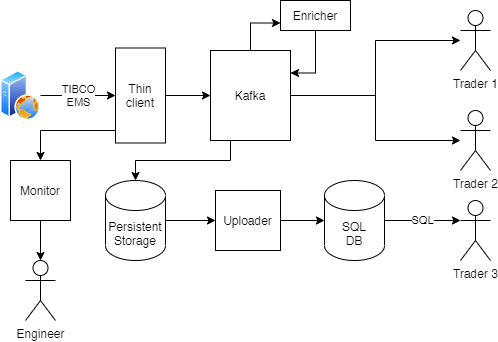
\includegraphics[width=1.0\columnwidth]{Figures/ArchitectureDiagram.png}
	\rule{35em}{0.5pt}
	\caption[Architecture Diagram]{Architecture Diagram of proposed system}
	\label{fig:Architecture Diagram}
\end{figure}
%----------------------------------------------------------------------------------------
%	SECTION 1
%----------------------------------------------------------------------------------------

	%\input{Chapters/Chapter4}
	%\input{Chapters/Chapter5}
	%\input{Chapters/Chapter6}
	%\input{Chapters/Chapter7}
	
	%-------------------------------------------------------------------------------
	%	THESIS CONTENT - APPENDICES
	%-------------------------------------------------------------------------------
	
	\addtocontents{toc}{\vspace{2em}} % Add a gap in the Contents, for aesthetics
	
	\appendix % Cue to tell LaTeX that the following 'chapters' are Appendices
	
	% Include the appendices of the thesis as separate files from the Appendices
	% folder
	% Uncomment the lines as you write the Appendices
	
	% Appendix A

\chapter{Institutional Brokers' Estimate System} % Main appendix title

\label{AppendixA} % For referencing this appendix elsewhere, use \ref{AppendixA}

\lhead{\emph{I/B/E/S}} % This is for the header on each page - perhaps a shortened title

The Institutional Brokers' Estimate System (I/B/E/S) is a service founded by the New York brokerage firm Lynch, Jones and Ryan and Technimetrics, Inc. I/B/E/S began collecting earnings estimates for U.S. companies around 1976 and used the raw data to calculate statistical time series for each company. The data subsequently was used as the basis for articles in academic finance journals attempting to demonstrate that changes in consensus earnings estimates could identify opportunities to capture excess returns in subsequent periods. After starting with annual earnings estimates and estimates of "Long Term Growth, the database later was expanded to include quarterly earnings estimates. This allowed for the analysis of "Quarterly Earnings Surprises." Other innovations made possible by the I/B/E/S data included estimates for various equity indexes on a "top down" basis (made by strategists and economists) and estimates made on a "bottom up" basis (by individual analysts) for those same indexes. In the mid-1980s I/B/E/S began to expand its dataset to include companies trading in international markets. Lynch, Jones was sold to Citigroup in 1986. Barra bought I/B/E/S in 1993, selling it to Primark two years later. Thomson Financial purchased Primark in 2000. Successor companyThomson Reuters spun off its financial division under the name Refinitiv in 2018.

The I/B/E/S database currently covers over 40,000 companies in 70 markets. It provides to a client base of 50,000 institutional money managers. More than 900 firms contribute data to I/B/E/S, from the largest global houses to regional and local brokers, with US data back to 1976 and international data back to 1987.
	%\input{Appendices/AppendixB}
	%\input{Appendices/AppendixC}
	
	\addtocontents{toc}{\vspace{2em}} % Add a gap in the Contents, for aesthetics
	
	\backmatter
	
	%-------------------------------------------------------------------------------
	%	BIBLIOGRAPHY
	%-------------------------------------------------------------------------------
	
	\label{Bibliography}
	
	\lhead{\emph{Bibliography}} % Change the page header to say "Bibliography"
	
	\printbibliography
	
\end{document}
